\chapter{Simple parent-daughter pairs}
\label{ch:intro2PD}

\section{$^{14}$C dating}
\label{sec:14C}

There are two stable isotopes of carbon: $^{12}$C and $^{13}$C, and
one naturally occurring radionuclide: $^{14}$C. The half life of
$^{14}$C is only 5,730 years, which is orders of magnitude shorter
than the age of the Earth. Therefore, no primordial radiocarbon
remains and all $^{14}$C is \emph{cosmogenic}\ifuclnotes (see Section
\ref{sec:cosmo} for related methods)\fi.  The main production
mechanism is through secondary cosmic ray neutron reactions with
$^{14}$N in the stratosphere: $^{14}_7$N (n,p) $^{14}_6$C. Any newly
formed $^{14}$C rapidly mixes with the rest of the atmosphere creating
a spatially uniform carbon composition, which is incorporated into
plants and the animals that eat them. Prior to the industrial
revolution, a gram of fresh organic carbon underwent 13.56 ($\beta^-$)
decays per minute. When a plant dies, it ceases to exchange carbon
with the atmosphere and the $^{14}$C concentration decays with time
according to Equation \ref{eq:dPdt}:

\begin{equation}
\frac{d^{14}C}{dt} = -\lambda_{14} \times {}^{14}C
\label{eq:d14Cdt}
\end{equation}

where $\lambda_{14}$ = 0.120968 kyr$^{-1}$. Thus, the radiocarbon
concentration is directly proportional to the radioactivity, which can
be measured by $\beta$-counting. This can then be used to calculate
the radiocarbon age by rearranging Equation \ref{eq:P}:

\begin{equation}
t = -\frac{1}{\lambda_{14}}
\ln\left[\frac{d{}^{14}C/dt}{(d{}^{14}C/dt)_\circ}\right]
\label{eq:t14C}
\end{equation}

where $(d^{14}C/dt)_\circ$ is the original level of $\beta$ activity.
This method was developed by Willard Libby in 1949, for which he was
awarded the Nobel Prize in 1960. As mentioned before,
$(d^{14}C/dt)_\circ$ was 13.56 prior to the industrial revolution,
when thousands of tonnes of `old' carbon were injected into the
atmosphere, resulting in a gradual lowering of the radiocarbon
concentration until 1950, when nuclear testing produced an opposite
effect, leading to a doubling of the atmospheric $^{14}$C activity in
1963. Since the banning of atmospheric nuclear testing, radiocarbon
concentrations have steadily dropped until today, where they have
almost fallen back to their pre-industrial levels. But even prior to
these anthropogenic effects, $^{14}$C concentrations underwent
relatively large fluctuations as a result of secular variations of the
Earth's magnetic field and, to a lesser extent, Solar activity. These
variations in $(d^{14}C/dt)_\circ$ can be corrected by comparison with
a precisely calibrated production rate curve, which was constructed by
measuring the $^{14}$C activity of tree rings
(\emph{dendrochronology}).\\

Since the 1980's, $\beta$-counting has been largely replaced by
accelerator mass spectrometry (AMS, see Section \ref{sec:mass-specs}),
in which the $^{14}$C concentration is measured directly relative to a
stable isotope such as $^{13}$C. Although this has not significantly
pushed back the age range of the radiocarbon method, it has
nevertheless revolutionised the technique by reducing the sample size
requirements by orders of magnitude. It is now possible to analyse
individual seeds or tiny fragments of precious objects such as the
Turin Shroud, which was dated at AD1260-1390.

\section{The Rb-Sr method}
\label{sec:Rb-Sr}

Trace amounts of Rb and Sr are found in most minerals as substitutions
for major elements with similar chemical properties. Rb is an alkali
metal that forms single valent positive ions with an ionic radius of
1.48 \AA, which is similar to K$^+$ (1.33 \AA).  Rb is therefore
frequently found in K-bearing minerals such as micas, K-feldspar and
certain clay minerals. Strongly evolved alkalic rocks such as
syenites, trachites and rhyolites often contain high Rb
concentrations.  Rb contains two isotopes of constant abundance:
$^{85}$Rb (72.1854\%) and $^{87}$Rb (27.8346\%). Sr is an alkaline
earth metal that forms bivalent positive ions with a radius of 1.13
\AA, similar to Ca$^{2+}$ (ionic radius 0.99 \AA). It therefore
substitutes Ca$^{2+}$ in many minerals such as plagioclase, apatite,
gypsum and calcite in sites with 8 neighbours, but not in pyroxene
where Ca$^{2+}$ has a coordination number of 6. Native Sr$^{2+}$ can
also substitute K$^+$ in feldspars (where radiogenic Sr is expected to
be found), but this substitution is limited and requires the
simultaneous replacement of Si$^{4+}$ by Al$^{3+}$ in order to
preserve electric neutrality.  Sr therefore predominantly occurs in
Ca-rich undifferentiated rocks such as basalts. Sr contains four
isotopes ($^{84}$Sr, $^{86}$Sr, $^{87}$Sr and $^{88}$Sr) with variable
abundance due to the variable amount of radiogenic $^{87}$Sr. However,
the non-radiogenic $^{84}$Sr/$^{86}$Sr and $^{86}$Sr/$^{88}$Sr-ratios
are constant with values of 0.056584 and 0.1194, respectively. The
Rb-Sr chronometer is based on the radioactive decay of $^{87}$Rb to
$^{87}$Sr:

\begin{equation}
{}^{87}Rb \rightarrow {}^{87}Sr + \beta^- + \nu +
0.275 MeV
\label{eq:87Rb}
\end{equation}

Where $\nu$ indicates an antineutrino. The number of radiogenic
${}^{87}$Sr atoms produced by this reaction after a time t is given
by:

\begin{equation}
{}^{87}Sr^* = {}^{87}Rb (e^{\lambda_{87} t} - 1)
\label{eq:87Sr*}
\end{equation}

where $^{87}Rb$ is the actual number of $^{87}$Rb atoms per unit
weight and $\lambda_{87}$ is the decay constant 1.42 $\times$
10$^{-11}$ yr$^{-1}$ (t$_{1/2}$ = 4.88$\times$10$^{10}$yr).  In
addition to this radiogenic $^{87}$Sr, most samples will also contain
some `ordinary' Sr. The total number of $^{87}$Sr atoms measured is
therefore given by:

\begin{equation}
^{87}Sr = {}^{87}Sr^* + {}^{87}Sr_\circ
\label{eq:87Sr}
\end{equation}

with $^{87}Sr_\circ$ the initial $^{87}$Sr present at the time of
isotopic closure.  Combining Equations \ref{eq:87Sr} and
\ref{eq:87Rb}, we obtain:

\begin{equation}
^{87}Sr = {}^{87}Sr_\circ + {}^{87}Rb (e^{\lambda_{87} t} - 1)
\label{eq:87Sr2}
\end{equation}

Dividing this by the non-radiogenic $^{86}$Sr yields

\begin{equation}
\frac{^{87}Sr}{^{86}Sr} =
\left(\frac{^{87}Sr}{^{86}Sr}\right)_\circ +
\frac{^{87}Rb}{^{86}Sr} (e^{\lambda_{87} t} - 1)
\label{eq:87Sr86Sr}
\end{equation}

The method can be applied to single minerals or to whole rocks.  Given
the very long half life, the optimal time scale ranges from the
formation of the solar system to the late Palaeozoic (300-400 Ma).  To
measure a Rb/Sr age, the weight percentage of Rb is measured by means
of X-ray fluorescence, ICP-OES or similar techniques, and the
$^{87}$Sr/$^{86}$Sr ratio is determined by mass spectrometry (isotope
dilution). The $^{87}$Rb/$^{86}$Sr-ratio is then calculated as:

\begin{equation}
\frac{^{87}Rb}{^{86}Sr} =
\frac{Rb}{Sr} \frac{Ab(^{87}Rb)
  M(Sr)}{Ab(^{86}Sr) M(Rb)}
\label{eq:87Rb86Sr}
\end{equation}

Where $Ab(\cdot)$ signifies `abundance' and $M(\cdot)$ `molar mass'.

\section{Isochrons}
\label{sec:isochrons}

Equation \ref{eq:87Rb86Sr} can be used in one of two ways. A first
method is to use an assumed value for $(^{87}$Sr$/^{86}$Sr)$_\circ$,
based on the geological context of the sample. This method is only
reliable for samples with a high Rb/Sr ratio (e.g., biotite) because
in that case, a wrong value for $({}^{87}$Sr$/{}^{86}$Sr$)_\circ$ has
only a minor effect on the age. A second and much better method is to
analyse several minerals of the same sample and plot them on a
$(^{87}$Rb$/^{86}$Sr) vs.  (${}^{87}$Sr$/{}^{86}$Sr) diagram (Figure
\ref{fig:isochron}).  Due to Equation \ref{eq:87Sr86Sr}, this should
form a linear array (the so-called \emph{isochron}) with slope
$(e^{\lambda_{87} t} - 1)$ and intercept
$({}^{87}Sr/{}^{86}Sr)_\circ$.  Both parameters can be determined
by linear regression, allowing us to quantify the `goodness of fit' of
the data and obviating the need to assume any initial Sr-ratios.

\ifpdf
\ifuclnotes
\begin{figure}[!ht]
  \centering
  \def\svgwidth{.7\textwidth}
  \input{isochron.pdf_tex}
  \caption{Schematic evolution of the $^{87}$Sr$/{}^{86}$Sr-system as
    a function of time for multiple aliquots of a hypothetical sample
    with initial ratio $({}^{87}$Sr$/{}^{86}$Sr$)_\circ$=0.700. The
    slope of the isochron is a function of the age as per Equation
    \ref{eq:87Sr86Sr} \citep[modified from][]{allegre2008}.}
  \label{fig:isochron}
\end{figure}
\else % end of uclnotes
\begin{figure}[!ht]
\noindent\begin{minipage}[t]{.6\textwidth}
\strut\vspace*{-\baselineskip}\newline
\def\svgwidth{\textwidth}
\input{isochron.pdf_tex}
\end{minipage}
\begin{minipage}[t]{.4\textwidth}
  \captionof{figure}{Schematic evolution of the $^{87}$Sr$/{}^{86}$Sr-system as
    a function of time for multiple aliquots of a hypothetical sample
    with initial ratio $({}^{87}$Sr$/{}^{86}$Sr$)_\circ$=0.700. The
    slope of the isochron is a function of the age as per Equation
    \ref{eq:87Sr86Sr} \citep[modified from][]{allegre2008}.}
  \label{fig:isochron}
\end{minipage}
\end{figure}
\fi % end of pdf
\else
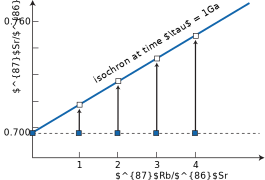
\includegraphics[width=10cm]{../figures/isochron.png}
  \captionof{figure}{Schematic evolution of the $^{87}$Sr$/{}^{86}$Sr-system as
    a function of time for multiple aliquots of a hypothetical sample
    with initial ratio $({}^{87}$Sr$/{}^{86}$Sr$)_\circ$=0.700. The
    slope of the isochron is a function of the age as per Equation
    \ref{eq:87Sr86Sr} \citep[modified from][]{allegre2008}.}
  \label{fig:isochron}
\fi

\section{The Sm-Nd method}
\label{sec:Sm-Nd}

The elements Neodymium (Z=60) and Samarium (Z=62) are so-called `rare
earth elements'.  All elements of this family have similar chemical
properties. They nearly all form 3+ ions of roughly equal albeit
slightly decreasing size with atomic number.  The ionic radius of Nd
and Sm is 1.08 and 1.04 \AA, respectively.  As the name suggests, rare
earth elements rarely form the major constituents of minerals.  One
notable exception is monazite, which is a rare earth phosphate. In
most cases, the rare earth elements are found in trace amounts of up
to 0.1\% in apatite [Ca$_5$(PO$_4$)$_3$(OH,Cl,F)] and zircon
[ZrSiO$_4$]. Both Sm and Nd are slightly enriched in feldspar, biotite
and apatite and thus tend to be found in higher concentrations in
differentiated (alkalic) magmatic rocks.\\

Because their chemical properties are so similar, geological processes
are rarely capable of fractionating the Sm and Nd
concentrations. Therefore, the Sm/Nd ratio in most rocks generally
falls in a narrow range of 0.1 to 0.5 (the Sm/Nd ratio of the solar
system being 0.31). One exception is garnet, in which Sm/Nd ratios $>$
1 have been found. Partial melting of mafic minerals such as pyroxene
and olivine produces lower Sm/Nd ratios in the fluid phase than the
solid residue.  The Sm/Nd ratio of magmatic rocks therefore decreases
with increasing differentiation.\\

Natural Sm contains seven naturally occurring isotopes, three of which
are radioactive ($^{147}$Sm, $^{148}$Sm and $^{149}$Sm). Only
$^{147}$Sm has a sufficiently short half life to be useful for
geochronology.  Nd also contains seven isotopes, of which only one is
radioactive ($^{144}$Nd) but with a very long half life. $^{143}$Nd is
the radiogenic daughter of $^{147}$Sm and is formed by
$\alpha$-decay. This forms the basis of the Sm-Nd chronometer.
Analogous to the Rb-Sr method (Equation \ref{eq:87Sr*}), we can write:

\begin{equation}
^{143}Nd^* = {}^{147}Sm (e^{\lambda_{147} t} - 1)
\label{eq:144Nd*}
\end{equation}

Hence:

\begin{equation}
t = \frac{1}{\lambda_{147}}
\ln\left(\frac{^{143}Nd^*}{^{147}Sm} + 1 \right)
\label{eq:tNd}
\end{equation}

With $\lambda_{147}$ = 6.54$\times$10$^{-12} $yr$^{-1}$ ($t_{1/2}$ =
1.06$\times$10$^{11}$yr).  Since most samples contain some initial Nd,
the preferred way to calculate Sm/Nd ages is by analysing several
minerals in a rock and create an isochron, similar to the Rb/Sr method
(Section \ref{sec:isochrons}):

\begin{equation}
\frac{^{143}Nd}{^{144}Nd} =
\left(\frac{^{143}Nd}{^{144}Nd}\right)_{\circ} +
\frac{^{147}Sm}{^{144}Nd} \left(e^{\lambda_{147}t} -
1\right)
\label{eq:143Nd147Nd}
\end{equation}

All measurements are done by mass spectrometry using isotope dilution.
Because of the identical atomic masses of $^{147}$Sm and $^{147}$Nd,
it is necessary to perform a chemical separation between Sm and Nd
prior to analysis.\\

The Sm/Nd method is generally applied to basic and ultrabasic igneous
rocks (basalt, peridotite, komatiite) of Precambrian to Palaeozoic
age. The method thus complements the Rb/Sr method, which is
preferentially applied to acidic rock types. The Sm/Nd method can also
be applied to high grade metamorphic rocks (granulites, eclogites) as
well as meteorites (shergottites, nahklites). Since the rare earths
are significantly less mobile than Rb and Sr, the Sm/Nd is more
reliable in rocks that have been disturbed by weathering or
metamorphism.
